\begin{figure}[!t]
\begin{subfigure}{0.495\textwidth}
\centering
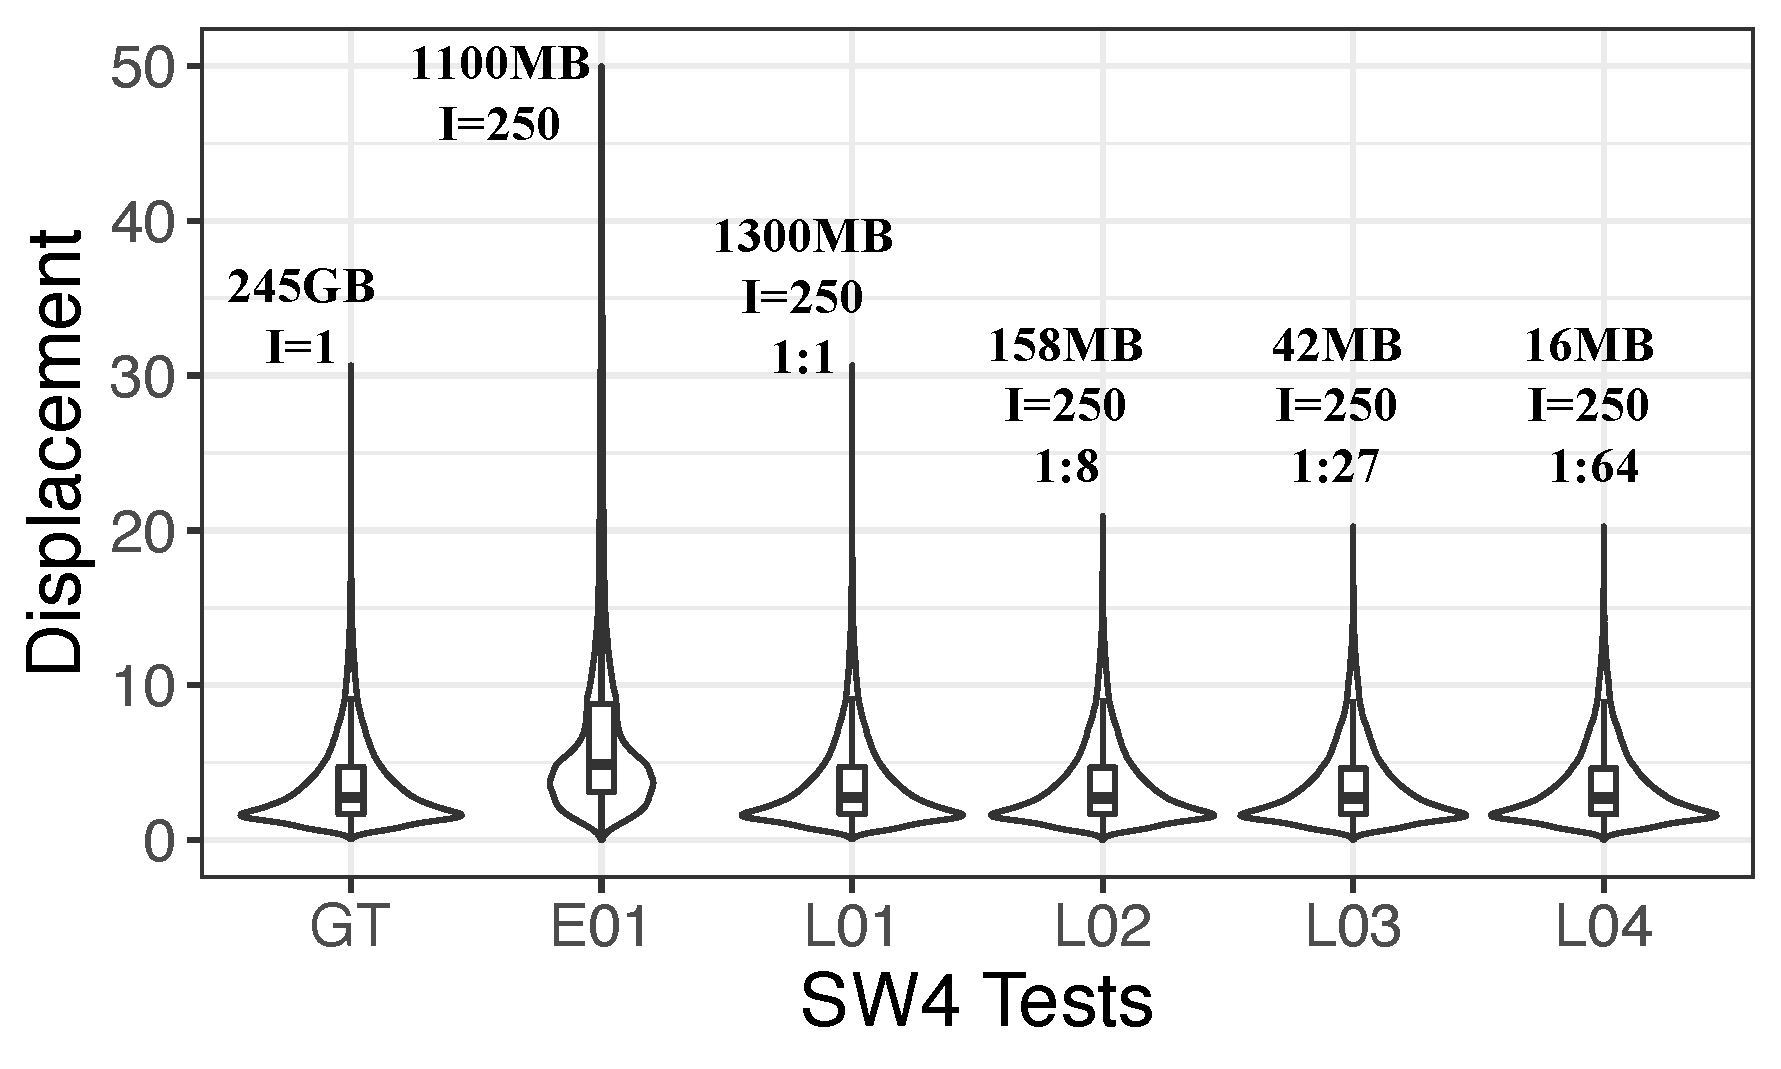
\includegraphics[width=\linewidth]{Images/sw4_violinplot1.pdf}
\vspace{-5mm}
\caption{High displacement near the epicenter.}
\label{fig:epicenter}
\end{subfigure}
\begin{subfigure}{0.495\textwidth}
\centering
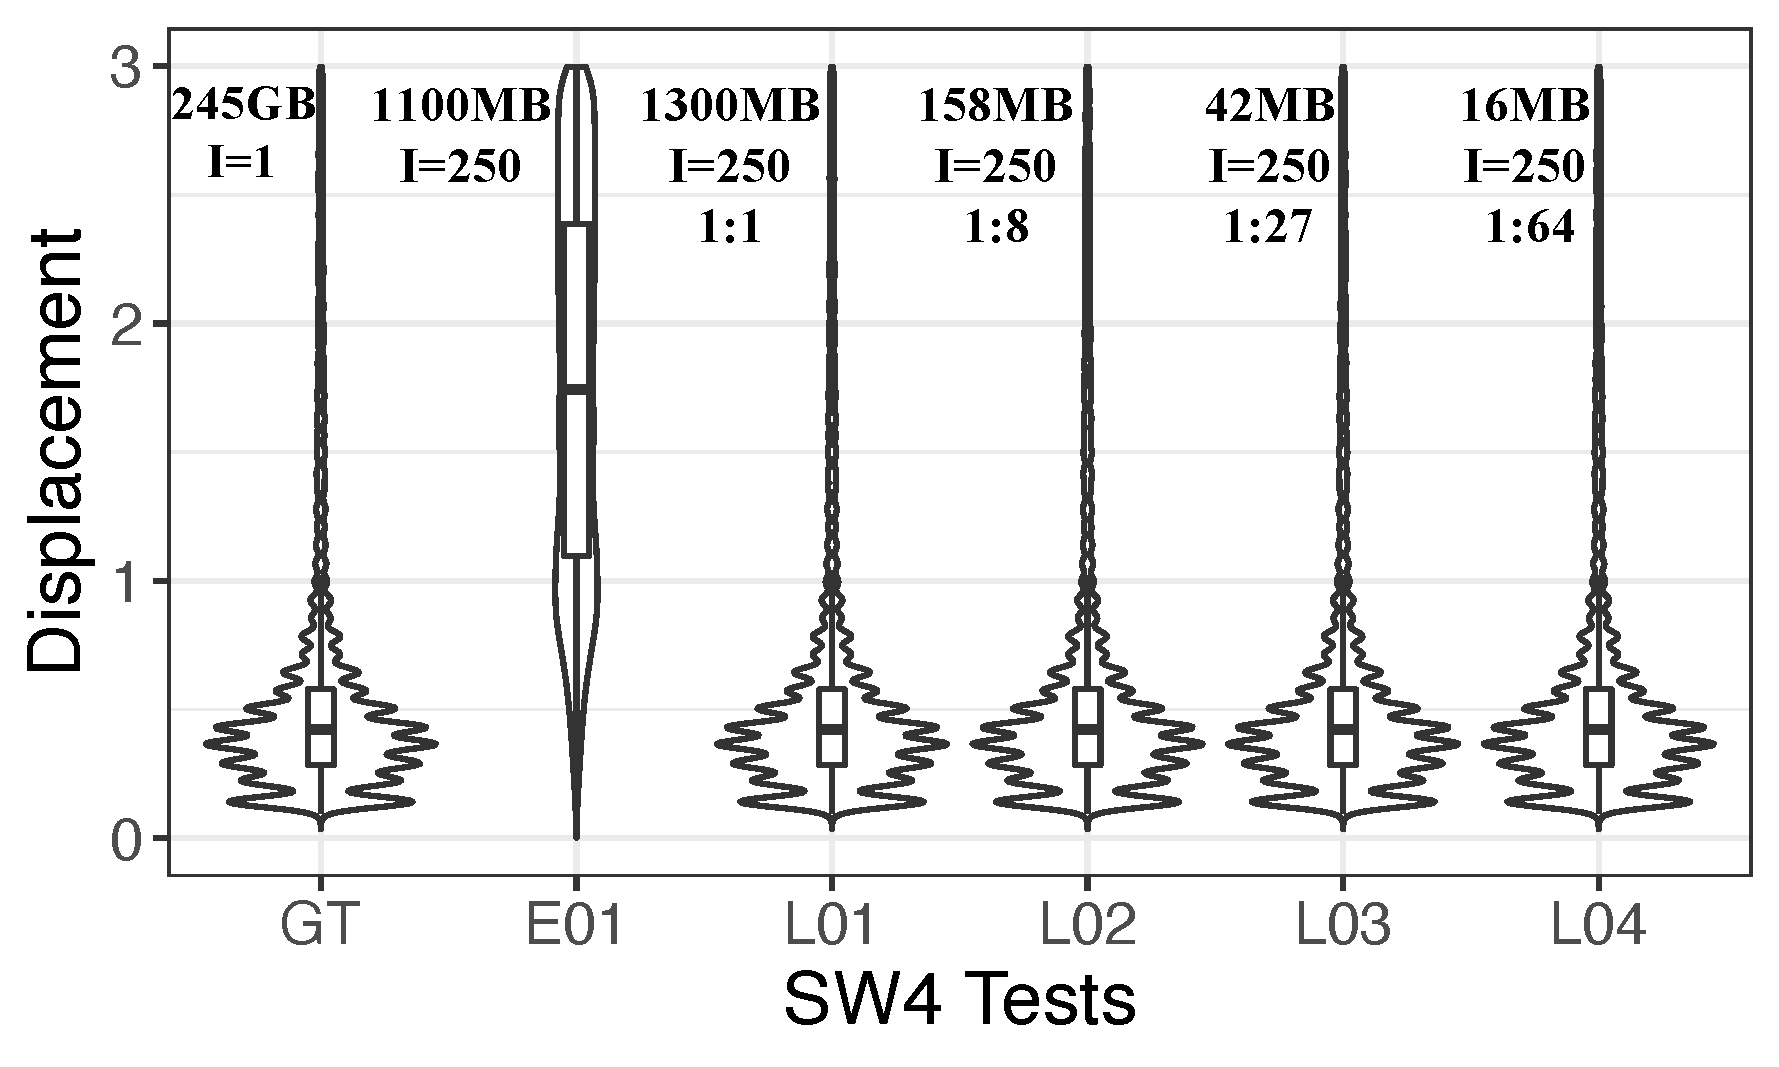
\includegraphics[width=\linewidth]{Images/sw4_violinplot2.pdf}
\vspace{-5mm}
\caption{Low displacement away from the epicenter.}
\label{fig:clusters}
\end{subfigure}
\vspace{-2mm}
\caption{Violin plots of distribution of particle displacement for the ground truth (GT), 1 Eulerian configuration and 4 Lagrangian configurations. The Eulerian configuration with access to limited number of time slices, overestimates the displacement. The Lagrangian representation encoding time intervals more accurately capture displacement in both setttings, in regions near and away from the epicenter.}
\vspace{-5mm}
\label{fig:sw4_violinplot}
\end{figure}
